\documentclass[14pt]{extreport}
\usepackage[framemethod=TikZ]{mdframed}
\usepackage{amsthm}
\usepackage{tcolorbox}
\usepackage[letterpaper, margin=1in]{geometry}
\usepackage{setspace}
\usepackage{amsmath}
\usepackage{cancel}
\usepackage{multicol}
\def\deg{\ensuremath{^\circ}}
\def\v#1{\ensuremath{\mathrm{#1}}}
\usepackage{multirow}
\usepackage{fancyhdr}
\pagestyle{fancy}
\usepackage{lastpage} 
\usepackage{colortbl}
\usepackage{amssymb}
\usepackage{graphicx}
\setlength{\parskip}{0pt}
\lhead{April 7, 2021}
\chead{}
\rhead{Source: Brilliant}

\lfoot{Jhon Christian N. Rozano}
\cfoot{}
\rfoot{Page \thepage\ of \pageref{LastPage}}

\renewcommand{\headrulewidth}{1pt}

\renewcommand{\footrulewidth}{1pt}

\newcommand*\Eval[3]{\left.#1\right\rvert_{#2}^{#3}}

\definecolor{LightCyan}{rgb}{0.88,1,1}
	


\begin{document}
	\setlength{\columnsep}{10pt}
	\renewcommand{\arraystretch}{1.5}
	\singlespacing
	
	\begin{center}
		{\large  \textbf{Physics Problem of the Day}} \\
		{\emph{Topic: Kinetic Energy}} 
	\end{center}
	
	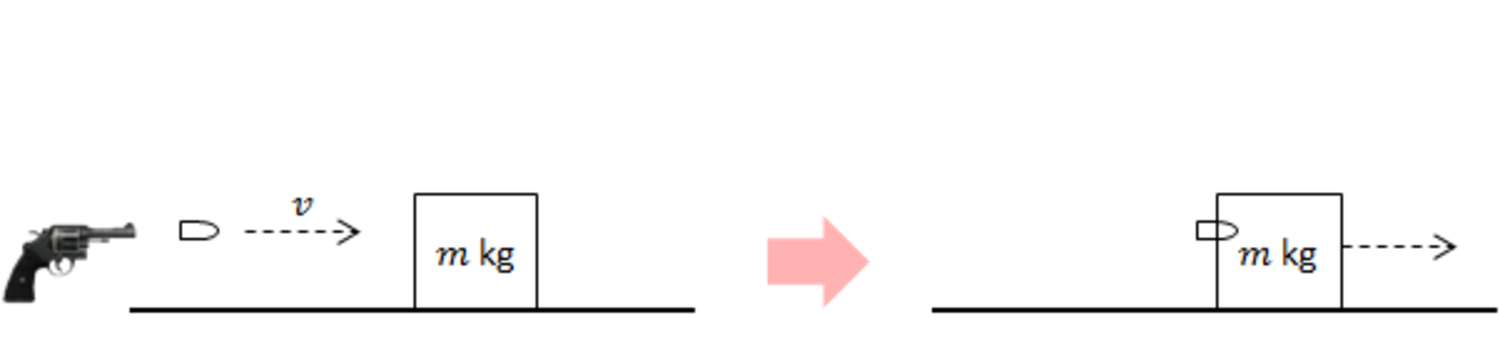
\includegraphics[scale=0.4, clip=true, trim=0mm 0mm 0mm 40mm]{39fe3a03d6.ffde83c235.28Ni7K.png}
	
	\noindent A wooden block of mass 4.8\text{ kg} is at rest on a frictionless floor. A bullet of mass 0.2\text{ kg} is fired at 800\text{ m/s} towards the block. If the bullet becomes embedded inside the block, how much kinetic energy is lost? \\
	
	\newtcolorbox{mybox}[1]{title=#1}
		\begin{mybox}{\textbf{Solution}}
			Since the question is asking for the lost kinetic energy, we should find the initial and final kinetic energy before and after the collision, respectively. Getting the initial kinetic energy gives us,
			
			\[ K_i = \frac{1}{2} \times ( 0.2\text{ kg} ) \times {( 800\text{ m/s} )}^2 = 64,000\text{ J} \]
			
			For the momentum, the law of conservation of momentum states that the initial momentum \( p_i \) is equal to the final momentum \( p_f \) of the system, and note that the scenario above is a perfectly inelastic collision, so we have
			
			\[ p_i = p_f \]
			\[ (m_1)({v_1}_i)+(m_2)({v_2}_i) = (m_1+m_2)(v_f)   \]
			\[ \left(  0.2\text{ kg} \right) \left( 800\text{ m/s} \right) + 0 = \left( 0.2\text{ kg} + 4.8\text{ kg}  \right)v  \] 
			\[ v = \text{32}\text{ m/s}   \]
			
			The final kinetic energy after the collision is given by
			
			\[ K_f = \frac{1}{2} \times \left( 0.2\text{ kg} + 4.8\text{ kg} \right) \times {( 32\text{ m/s}  )}^2 = 2560\text{ J}  \]
			
			Therefore, the lost in kinetic energy is
			
			\[ K_i - K_f = 64,000\text{ J} - 2560\text{ J} = \fbox{61440\text{ J}}\]
			
			
		\end{mybox}
	
\end{document}
